%%%%%%%%%%%%%%%%%%%%%%%%% 
% Dokumentinformationen % 
%%%%%%%%%%%%%%%%%%%%%%%%% 
\title{TSM\_PredMod}
\author{R. Ammann, D. Wright} % Do not remove any names!
% Initial authors stay first.
%\newcommand{\versioninfo}{FS2018}

\documentclass[10pt,twoside,a4paper,fleqn]{scrartcl}

%%%%%%%%%%%%%%%%%%%%%%%%%%%%%%%%%%%%%%%%%%%%%
% Standard projektübergreifender Header für
% - Makros 
% - Farben
% - Mathematische Operatoren  
%
% DORT NUR ERGÄNZEN, NICHTS LÖSCHEN
%%%%%%%%%%%%%%%%%%%%%%%%%%%%%%%%%%%%%%%%%%%%%  
\include{./header/zusammenfassung}

\usepackage{longtable}
%%%%%%%%%%%%%%%%%%%%%%%%%%%%%%%%%%%%%%%%%%%%%%%%%%%%%%%%%%%%%
% Additional commands and environments for this cheat sheet % 
%%%%%%%%%%%%%%%%%%%%%%%%%%%%%%%%%%%%%%%%%%%%%%%%%%%%%%%%%%%%%

% creates a pre-formatted two column table for arbitrary inputs 
\newenvironment{twoColTable}
{
	\begin{longtable}{|p{0.475\linewidth}|p{0.475\linewidth}|}%
	}%
	{%
	\end{longtable}%
}

\newcommand{\twoColHdrRow}[1]
{%
	\rowcolor{HSRBlue40}\multicolumn{2}{|l|}{\textbf{#1}}
}

\newcommand{\twoColHdrCell}[1]
{%
	\cellcolor{HSRBlue40}\textbf{#1}
}


% Creates a pre-formatted two column table with a code example column
% to the left, a command line output column to the right, and an 
% interpretation row for the command line output at the bottom
\newcommand{\RExample}[3]
{%
	\begin{twoColTable}
		\hline
		\twoColHdrCell{Source code:}
			&	\twoColHdrCell{Output:}\\*
		\hline
		\endhead
		\vspace{0pt}

		{\lstinputlisting[style=R]{#1}}% <-- source code here (1st argument: path to source code file (.R))
			&
			\vspace{0pt}

			{\lstinputlisting[style=R]{#2}}\\% <-- output here (2nd argument: path to output file (.R))
		\hline
		\twoColHdrRow{\textbf{Interpretation of output:}}\\*
		\hline
		\multicolumn{2}{|l|}{#3}\\
		\hline
	\end{twoColTable}%
}

% Creates a pre-formatted two column table with a theory column
% to the left, a code example column to the right
\newcommand{\RTheory}[2]
{%
	\begin{twoColTable}
		\hline
		\twoColHdrCell{Theory}
			& \twoColHdrCell{Code Example}\\*
		\hline
		\endhead
		#1% <-- Theory here (1st argument: theory, entered directly in the call to the command)
			&
				\vspace{0pt}

				{\lstinputlisting[style=R]{#2}}\\% <-- source code here (2nd argument: path to source code file containing a short example (.R))
		\hline
	\end{twoColTable}%
}

%%%%%%%%%%%%
% Document % 
%%%%%%%%%%%%
\begin{document} 

\selectlanguage{ngerman}
\section{R Tutorial}

\RCode{Help Function}{sections/RTutorial/help.R}

\RCode{Loading Data}{sections/RTutorial/loadingData.R}

\RCode{Function Definition}{sections/RTutorial/functions.R}



\section{Probability And Statistics}

\subsection{Probability Models for Measurement Data}
\subsubsection{Random Variables}
		{
			% Extra row height for fractions and integrals
			\setlength{\extrarowheight}{3pt}
		
			\begin{twoColTable}
				\hline
				\twoColHdrRow{Random Variables}\\
				\hline
				\textbf{Definition}
					& $X:\Omega \longrightarrow W\textsubscript{x}$\\
				\hline	
				\textbf{Example}
					& A Coin is thrown three times, head and tails is observed:\\
					& $\Omega = \left\{hhh, hht, htt, hth, ttt, tth, thh, tht\right\}$\\
					& Total number of heads $W\textsubscript{x}=\left\{0,1,2,3\right\}$\\
					& Total number of tails $W\textsubscript{x}=\left\{0,1,2,3\right\}$\\
					& Number of heads minus tails $W\textsubscript{x}=\left\{-3,-1,1,3\right\}$\\
				\hline
				\hline
				\twoColHdrRow{Probability Mass Function}\\
				\hline
				\textbf{Definition}
					& The probability distribution of a discrete random variable:\\
					&$P(X = x)$\\
				\hline	
				\textbf{Example}
				&
				\begin{tabular}{l|l*{4}{c}r}
					x & 0 & 1 & 2 & 3 \\
					\hline
					$P(X = x)$ & $\frac{1}{8}$ & $\frac{3}{8}$ & $\frac{3}{8}$ & $\frac{1}{8}$\\
				\end{tabular}\\
				\hline	
			\end{twoColTable}
		}
		
	\subsubsection{Odds vs. Probability}
		\begin{twoColTable}
			\hline
			\twoColHdrCell{Odds}
				& \twoColHdrCell{Probability}\\
			\hline
			$o(x) \in [0, \inf)$
				& $p(x) \in [0, 1]$\\
			\hline
			$o(X=x) = \frac{\text{Number of events where }X=x}{\text{Number of events where }X \neq x}$
				& $p(X=x) = \frac{\text{Number of events where }X=x}{\text{Total number of events}}$\\
			\hline
			$o = \frac{p}{1-p}$
				& $p = \frac{o}{1+o}$\\			
			\hline
		\end{twoColTable}

	\subsubsection{Probability Distributions}
		{
			% Extra row height for fractions and integrals
			\setlength{\extrarowheight}{3pt}
		
			\begin{twoColTable}
				\hline
				\twoColHdrRow{Cumulative Density Function (cdf)}\\
				\hline
				\textbf{Definition}
					& $F(x) = P(X \leq x)$\\
				\hline	
				\textbf{Properties}
					& $P(a < X \leq b) = F(b) - F(a)$\\
					& $0 \leq F(x) \leq 1$\\
					& $P(X = a) = F(a) - F(a) = 0$\\
				\hline
			\end{twoColTable}

			\begin{twoColTable}
				\hline
				\twoColHdrRow{Probability Density Function (pdf)}\\
				\hline
				\textbf{Definition}
					& $ f(x) = \diff{F(x)}{x}$\\[1ex] % bottom padding for fraction
				\hline	
				\textbf{Properties}
					& $f(x) \geq 0$\\[1ex] % bottom padding for integral
					& $ P(a < X \leq b) = F(b) - F(a) = \int\limits_a^b f(x)\mathrm{d}x$\\[1ex] % bottom padding for integral
					& $\int\limits_{-\infty}^{\infty} f(x)\mathrm{d}x = 1$\\[1ex] % bottom padding for integral
				\hline
			\end{twoColTable}
		}
		
		\begin{figure}[H]\centering
			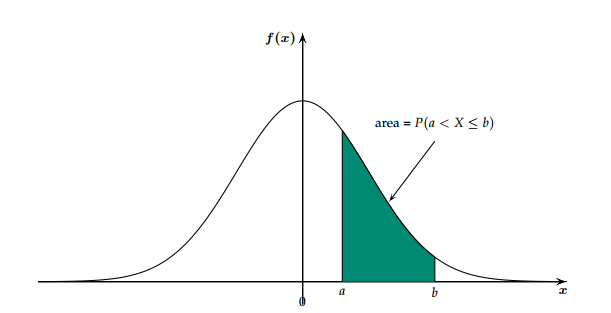
\includegraphics[scale=0.5]{images/ProbabilityDensityRV.png}
			\caption{Probability density of a random variable and the probability of measuring a value from (a,b]}
		\end{figure}
	
	\subsubsection{Summary Statistics of Continuous Distributions}
		{
			% Extra row height for fractions and integrals
			\setlength{\extrarowheight}{3pt}
			
			\begin{twoColTable}
				\hline
				\twoColHdrRow{Expected Value, Variance and Quantile}\\
				\hline
				\textbf{Expected value}
										& Discrete: $\mathrm{E}(X) = \sum\limits_{i} x_i P(X = x_i)$\\
										& Continuous: $\mathrm{E}(X) = \mu_X = \int\limits_{-\infty}^{\infty} x \cdot f(x) \mathrm{d}x$\\[1ex] % bottom padding for integral
				\hline
				\textbf{Variance}
					& $\mathrm{Var}(X) = \sigma_x^2 = \mathrm{E}((X - \mathrm {E}(X))^2) =  \int\limits_{-\infty}^{\infty} (x - \mathrm{E}(X))^2 \cdot f(x) \mathrm{d}x$\\[1ex] % bottom padding for integral
				\hline
				\textbf{Quantile}
					& $P(X \leq q(\alpha)) = \alpha$\\
					& $F(q(\alpha)) = \alpha \Leftrightarrow q(\alpha) = F^{-1}(\alpha)$\\
					& {\color{red}Note: When you're asked for the $50\%$-quantile, that means $\alpha = 50\%$, and you must find $q(0.5)$}\\
				\hline
				\textbf{Example Body Length}
				& If $\alpha$=0.75 and the corresponding quantile is $q(\alpha)$=182.5cm\\
				& then 75$\%$ of the persons is shorter or equal 182.5cm.\\
				\hline			 
			\end{twoColTable}
		}
		
		\begin{figure}[H]\centering
			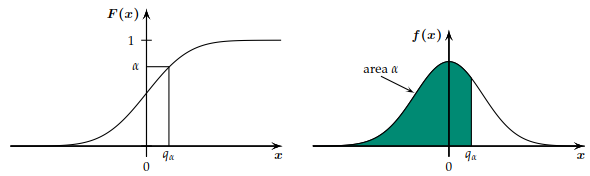
\includegraphics[scale=0.5]{images/quantile.png}
			\caption{Quantiles}
		\end{figure}
		
		\subsubsection{Important Distributions}
			\paragraph{Uniform Distribution}
				\RTheory%
				{%
					$$\begin{aligned}[t]
						f(x) 			&= 	\begin{cases}
												\frac{1}{b - a} 	& a \leq x \leq b\\
												0					& \mathrm{otherwise}\\ 
											\end{cases}\\
						F(x) 			&= 	\begin{cases}
												0					& x < a\\
												\frac{x-a}{b - a} 	& a \leq x \leq b\\
												1					& x > b\\ 
											\end{cases}\\
						\mathrm{E}(x) 	&= \frac{a+b}{2}\\
						\mathrm{Var}(x) &= \frac{(b-a)^2}{12}\\
						\mathrm{\sigma_x} &= \frac{b-a}{\sqrt{12}}\\
					\end{aligned}$$
				}{sections/ProbabilityStatistics/ProbabilityModels/ImportantDistributions/uniformTheory.R}
				
				\paragraph{Exponential Distribution}
				\RTheory%
				{%
					$$\begin{aligned}[t]
						f(x) 			&= 	\begin{cases}
												\lambda\cdot e^{-\lambda\cdot x} 	& x \geq 0\\
												0					& \mathrm{otherwise}\\ 
											\end{cases}\\
						F(x) 			&= 	\begin{cases}
												1- \lambda\cdot e^{-\lambda\cdot x} 	& x \geq 0\\
												0					& \mathrm{otherwise}\\ 
											\end{cases}\\
						\mathrm{E}(x) 	&= \frac{1}{\lambda}\\
						\mathrm{Var}(x) &= \frac{1}{\lambda^2}\\
					    \mathrm{\sigma_x} &= \frac{1}{\lambda}\\
					\end{aligned}$$
				}{sections/ProbabilityStatistics/ProbabilityModels/ImportantDistributions/exponentialTheory.R}
				\paragraph{Normal Distribution}
				\RTheory%
				{%
					$$\begin{aligned}[t]
						f(x) 			&=\frac{1}{{\sigma \sqrt {2\pi } }}e^{(- \frac{(x - \mu )^2 }{2\sigma ^2 })}\\
						F(x) 			&= 	 \int\limits_{-\infty}^{x} f(x)\mathrm{d}y \\
						\mathrm{E}(x) 	&= \mu \\
						\mathrm{Var}(x) &=\sigma^2 \\
					    \mathrm{\sigma_x} &= \sigma\\
					\end{aligned}$$
				}{sections/ProbabilityStatistics/ProbabilityModels/ImportantDistributions/gaussianTheory.R}
				\paragraph{Linear Transformation of Random Variables}
				{
			% Extra row height for fractions and integrals
			\setlength{\extrarowheight}{3pt}
		
			\begin{twoColTable}
				\hline
				\twoColHdrRow{Properties of Linear Transformation of a Random Variable}\\
				\hline
				\textbf{Definition}
					& For $ Y=a+bX$ the following apply\\
					&   (i) $E(Y)= a+bE(X)$\\
					&  (ii) $Var(Y)= b^2Var(X), \, \sigma_Y = |b|\sigma_X$\\
					& (iii) $\alpha-Quantile\,of\,Y = q_Y(\alpha) = a+bq_X(\alpha)$\\
					&  (iv) $f_Y(y) = \frac{1}{b}f_X(\frac{y-a}{b})$\\
				\hline
				\hline
				\twoColHdrRow{Summary Statistics of $S_n$ and $\bar{X}_n$}\\
				\hline
				\textbf{Summary Statistics of Sample Total $S_n$}
					& $E(S_n)=E(X_1+X_2+...+X_n)=\sum\limits_{i=1}\limits^{n}E(X_i)=n\mu$\\
					& $Var(S_n)=\sum\limits_{i=1}\limits^{n}Var(X_i)=nVar(X_i)$\\
					& $\sigma(S_n)=\sqrt{n}\sigma_X$\\
				\hline	
				\textbf{Summary Statistics of Sample Mean $\bar{X}_n$}
					& $E(\bar{X}_n)=E(\frac{X_1+X_2+...+X_n}{n})=\frac{1}{n}\sum\limits_{i=1}\limits^{n}E(X_i)=\frac{1}{n}nE(X_i)=\mu$\\
					& $ Var(\bar{X}_n)=\frac{1}{n^2}\sum\limits_{i=1}\limits^{n}Var(X_i)=\frac{1}{n^2}n\sigma_{X}^{2}=\frac{\sigma_{X}^{2}}{n}$\\
				\textit{Standard Error}
					& $\sigma(\bar{X}_n)=\frac{\sigma_X}{\sqrt{n}} $ \\
				\hline	
			\end{twoColTable}
		}
% 		\paragraph{Distributions of $S_n$ and $\bar{X}_n$}
% 				\RTheory%
% 				{%
% 				 1. For  $X_i \in \{ 0,1 \}$, we have
% 				 \begin{center}
% 				 $S_n \sim $Bin$(n,\pi)$ with $\pi = P(X_i=1)$\\
% 				 \end{center}
% 				 2. For $X_i \sim$Pois$(\lambda)$, we have
% 				 \begin{center}
% 				  $S_n \sim$Pois$(n\lambda)$\\
% 				 \end{center}				 
% 				 3. For $X_i \sim N(\mu,\sigma^2)$
% 				 \begin{center}
% 				  $S_n \sim N(n\mu,n\sigma^2)$ and $\bar{X}_n \sim N(\mu, \frac{\sigma_{X}^{2}}{n})$\\
% 				 \end{center}				 
% 				}{sections/ProbabilityStatistics/ProbabilityModels/ImportantDistributions/centralLimitTheorem.R}
\subsection{Statistics for Measurement Data}
	\subsubsection{Q-Q Plot}
		\RTheory
		{					
			1. For
			\begin{center}
				$\alpha_k=\frac{k-0.5}{n}$ with $k=1,...,n$\\
			\end{center}
			
			calculate the corresponding theoretical quantiles of the model distribution
			
			\begin{center}
				$q(\alpha_k)=F^{-1}(\alpha_k)$\\
			\end{center}				 
			
			2. Determine the empirical $\alpha_k$-quantiles,
			
			\begin{center}
				$x_{(1)}<x_{(2)}<...<x_{(n)}$\\
			\end{center}				 
			
			3. Plot the empirical quantiles $x_k$ on the y-axis against the theoretical quantiles 					$q(\alpha_k)$ on the x-axis.		 
		}
		{
			sections/ProbabilityStatistics/StatisticsForMeasurementData/RCode/QQPlot.R
		}
		
% 		\begin{figure}[H]
% 			\begin{minipage}[c]{0.5\textwidth}
% 				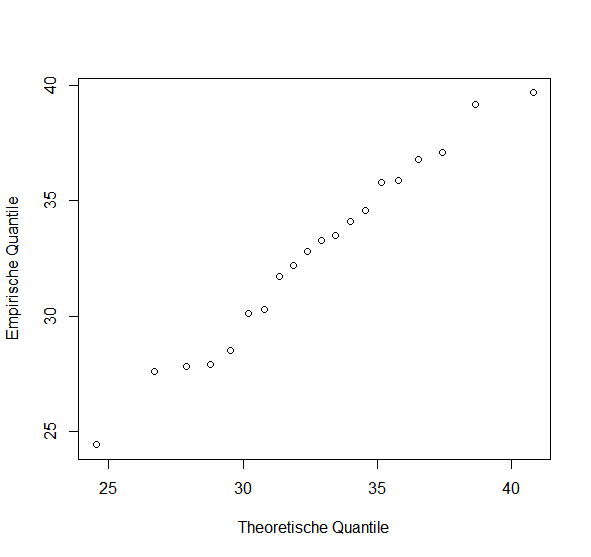
\includegraphics[width=1\linewidth]{images/qqPlot.png}
% 			\end{minipage}\hfill
% 			\begin{minipage}[c]{0.5\textwidth}
% 				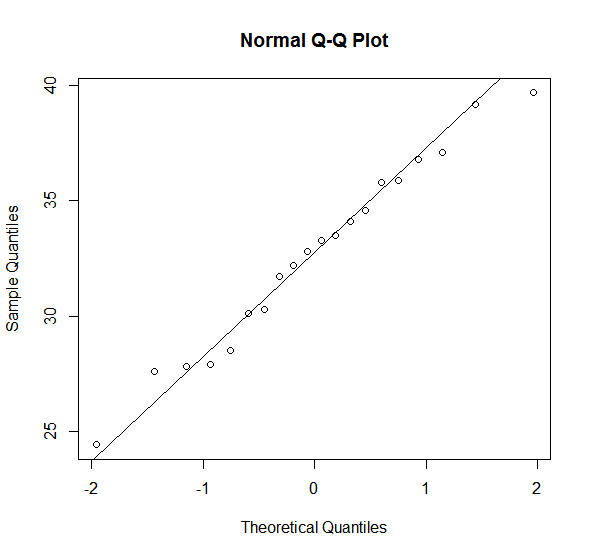
\includegraphics[width=1\linewidth]{images/qqNormLine.png}
% 			\end{minipage}\\
% 			\begin{minipage}[t]{.5\textwidth}
% 				\subcaption{qqplot()}
% 			\end{minipage}\hfill
% 			\begin{minipage}[t]{.5\textwidth}
% 				\subcaption{qqnorm();qqline()}
% 			\end{minipage}
% 		\end{figure}
% 		\begin{figure}[H]
% 			\begin{minipage}[c]{0.5\textwidth}
% 				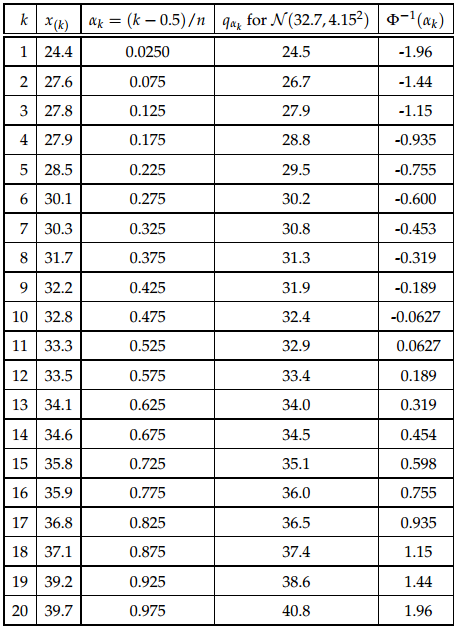
\includegraphics[width=1\linewidth]{images/qqList.png}
% 			\end{minipage}
% 			\begin{minipage}[c]{0.5\textwidth}
% 				\lstinputlisting[style=R]{sections/ProbabilityStatistics/StatisticsForMeasurementData/RCode/QQList.R}
% 			\end{minipage}
% 		\end{figure}

	\subsubsection{Parameter Esitmation for Continuous Probability Distributions}
	{
		% Extra row height for fractions and integrals
		\setlength{\extrarowheight}{3pt}
	
		\begin{twoColTable}
			\hline
			\twoColHdrRow{Method of Moments (not unbiased)}\\
			\hline
			\endhead
			Random variables							
				& $X_1,X_2,...,X_n$ \\
			\hline
			Measurements of these random variables (realisations, originating from same distribution)		
				& $x_1,x_2,...,x_n$ \\
			\hline
			Expected value
				& $\mu = E(X)  \Rightarrow \hat{\mu}=\bar{x}_n=\frac{x_1+x_2+...+x_n}{n}$\\
			\hline
			Variance
				& $\sigma^2 = E(X^2)-E(X)^2 = E(X^2)-\mu^2$\\
				& $\hat{\mu}^2+\hat{\sigma}^2 = \frac{1}{n}\sum\limits_{i=1}\limits^n x_i^2$\\
				& $\hat{\sigma}^2 = \frac{\sum\limits_{i=1}\limits^n(x_i-\bar{x}_n)^2}{n}$\\
				& $\hat{\sigma}^2 = \sqrt{\frac{1}{n}\sum\limits_{i=1}\limits^n(x_i-\hat{\mu})^2}$\\
			\hline
		\end{twoColTable}
		
		
		\begin{twoColTable}
			\hline
			\twoColHdrRow{Method of Maximum Likelihood}\\
			\hline
			General idea
				& Estimate a generic parameter (named $\theta$, which may represent $\mu$, $\lambda$\ldots) in such a way that the likelihood is maximized, that is, that it makes the observed data most likely or most probable.\\
			\hline
			$n$ observations of random variables, that are i.i.d.
				& $X_1=x_1,X_2=x_2,...,X_n=x_n$\\
			\hline
			\twoColHdrRow{Discrete probability distribution:}\\
			\hline
			Probability that random variable $X_i$ takes the value $x_i$
				& $P[X_i=x_i]$\\
			\hline
			Probability that the observations actually occurred
				& 
					{$\begin{aligned}
						&P[(X_1=x_1)\cap (X_2=x_2)\cap ... \cap (X_n=x_n)]\\
						&= P[X_1=x_1]\cdot P[X_2=x_2]\cdot ... \cdot P[X_n=x_n]\\
						&= \prod\limits_{i=1}\limits^n P[X_i = x_i]
					\end{aligned}$}\\
			\hline
			Generic probability distribution parameter (e.g. $\mu$, $\lambda$\ldots)
				& $\theta$\\
			\hline
			Likelihood function:\newline Probability that the $n$ measurements of independent random variables are observed.
				& 
					{$\begin{aligned}
						&L(\theta) = P[X_1=x_1|\theta]\cdot P[X_2=x_2|\theta]\cdot ... \cdot P[X_n=x_n|\theta]\\
						&= \prod\limits_{i=1}\limits^n P[X_i = x_i|\theta]
					\end{aligned}$}\\
			\hline
			Probability that random variable $X_i$ takes the value $x_i$, given parameter $\theta$
				& $P[X_i = x_i|\theta]$\\
			\hline
			\twoColHdrRow{Continuous probability distributions :}\\
			\hline
			Probability density function 
				& $f(x;\theta)$.\\
			\hline 
			Probability that each observation $x_i$ falls into its corresponding interval $[x_i , x_i + dx_i]$
				& $\prod\limits_{i=1}\limits^n f(x_i; \theta)dx_i$\\
			\hline
			Infinitesimal intervals $dx_i$ do not depend on the parameter value $\theta$, we omit them in the likelihood function
				& $\prod\limits_{i=1}\limits^n f(x_i; \theta)$\\
			\hline
			\twoColHdrRow{Example: Maximum Likelihood for Exponential Distribution}\\
			\hline
			Random variables
				& $X_1, X_2 . . . , X_n$ i.i.d. $\sim$ Exp($\lambda$)\\
			\hline
			Probability density function 
				& $f(x_i; \lambda) = \lambda e^{-\lambda x_i}$\\
			\hline
			Likelihood function for a given data set
				& $L(\lambda) = \prod\limits_{i=1}\limits^n \lambda e^{-\lambda x_i}$\\
			\hline
			Log likelihood function
				& $\log(L(\lambda)) = n \log(\lambda) - \lambda \sum\limits_{i=1}\limits^n x_i$\\
			\hline
			Derivative of the log likelihood function with respect to $\lambda$ and set it to $0$
				& $\frac{d \log(L(\lambda))}{d\lambda}=\frac{n}{\lambda}-\sum\limits_{i=1}\limits^n x_i \overset{!}{=} 0$\\
			\hline
			Maximum likelihood estimate
				& $\hat\lambda = \frac{n}{\sum\limits_{i=1}\limits^n x_i}=\frac{1}{\bar{x}}$\\
			\hline	
		\end{twoColTable}
	}

	\subsubsection{Statistical Tests and Confidence Interval for Normally Distributed Data}
	{
		% Extra row height for fractions and integrals
		\setlength{\extrarowheight}{3pt}
				
		\begin{twoColTable}
			\hline
			\twoColHdrRow{$z$-Test ($\sigma_x$ known)}\\
			\hline
					1. Model:
					& $X_1,...,X_n$ i.i.d. $\sim N(\mu, \sigma_{X}^2)$, $\sigma_X$ known\\
			\hline	
					2. Null hypothesis:
					& $H_0$:	$\mu=\mu_0$\\
					Alternative:
					& $H_A$:	$\mu \neq \mu_0$	(or $<$ or $>$)\\
			\hline	
					3. Test statistic:
					& $Z=\frac{(\bar{X}_n - \mu_0)}{\sigma_{\bar{X}_n}}=\frac{(\bar{X}_n - \mu_0)}{\sigma_{X_n}/\sqrt{n}}=\frac{\sqrt{n}(\bar{X}_n - \mu_0)}{\sigma_{X_n}}=\frac{observed-expected}{standard\,error}$\\
					Null distribution (assuming $H_0$ is true):
					&$Z \sim N(0,1)$\\
			\hline
					4. Significance level:
					& $\alpha$\\
			\hline
					5. Rejection region for the test statistic:
					& $K=(-\infty,z_{\frac{\alpha}{2}}] \cup [z_{1-\frac{\alpha}{2}}, \infty)$ with $H_A: \mu \neq \mu_0$, \vfill 
					$K=(-\infty,z_\alpha]$ with $H_A: \mu < \mu_0$, \vfill
					$K=[z_{1-\alpha}, \infty)$ with $H_A: \mu > \mu_0$\\
					where
					& $z_{\frac{\alpha}{2}} = \Phi^{-1}(\alpha/2)$\\
			\hline
					6. Test decision:
					& Check whether the observed value of the test statistic falls into the rejection region.\\
			\hline
		\end{twoColTable}
	
		\begin{figure}[H]
		    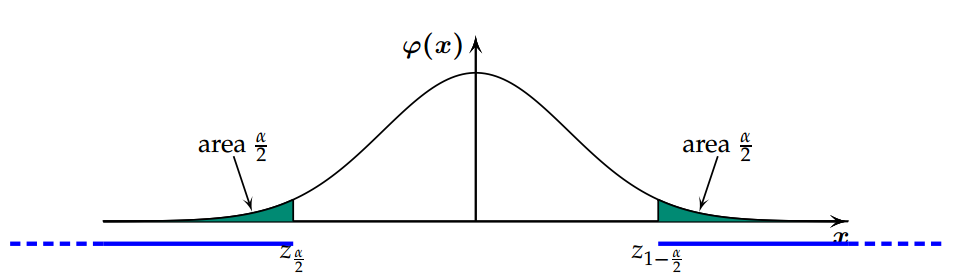
\includegraphics[width=0.5\linewidth]{images/zTestDecision.png}
		    \caption{z-Test: Rejection Region}
		\end{figure}
		
		\begin{twoColTable}
			\hline
			\twoColHdrRow{$z$-Test ($\sigma_x$ known): Standardized example}\\
			\hline
			Measurement of fusion heat:
				& The empirical mean value of $n=13$ measurements is $80.02$. From previous measurements the standard deviation is $\sigma_X = 0.01$. Is a fusion heat of exactly $80.00\frac{g}{cal}$ plausible?\\
			\hline
			Model:
				& $X_1,...,X_n$ i.i.d. $\sim N(\mu, \sigma_{X}^2)$, $\sigma_X=0.01$ known, $n=13$\\
			\hline	
			Null hypothesis:
				& $H_0$:	$\mu=\mu_0=80.00$\\
			Alternative:
				& $H_A$:	$\mu \neq \mu_0$\\
			\hline	
			Test statistic:
				& $Z=\frac{\sqrt{n}(\bar{X}_n - \mu_0)}{\sigma_{X_n}}$\\
			\hline
			Null distribution (assuming $H_0$ is true):
				&$Z \sim N(0,1)$\\
			\hline
			Significance level:
				& $\alpha = 0.05$ (commonly used $\alpha$-level)\\
			\hline
			Given $\alpha = 0.05$, {\color{blue}R} yields the following 2.5$\%$ quantile of the standard normal distribution.
				& {\lstinputlisting[style=R]{sections/ProbabilityStatistics/StatisticsForMeasurementData/RCode/zTest.R}}\\
			Rejection region for the test statistic (with the quantile returned from {\color{blue}R}):
				& 
					 {$\begin{aligned}
						z_{\frac{\alpha}{2}} &= \Phi^{-1}(\alpha/2) = \Phi^{-1}(0.025)=-1.96\\
						K &= (-\infty,z_{\frac{\alpha}{2}}] \cup [z_{1-\frac{\alpha}{2}}, \infty) \quad \mathrm{with} \quad H_A: \mu \neq \mu_0\\
						K &= (-\infty,-1.96] \cup [1.96, \infty)
					 \end{aligned}$}\\
			\hline
			Test decision:
				& $z=\frac{\sqrt{n}(\bar{X}_n - \mu_0)}{\sigma_{X_n}}=\frac{\sqrt{13}(80.02 - 80.00)}{0.01}=7.211$\\
				& Therefore the observed value falls into the rejection region.\\
			\hline
		\end{twoColTable}
			
		\begin{twoColTable}
			\hline
			\twoColHdrRow{$z$-Test ($\sigma_x$ known): Not standardized example}\\
			\hline
			Measurement of fusion heat:
				& The empirical mean value of $n=13$ measurements is $80.02$. From previous measurements the standard deviation is $\sigma_X = 0.01$. Is a fusion heat of exactly $80.00\frac{g}{cal}$ plausible?\\
			\hline
			Model:
				& $X_1,...,X_n$ i.i.d. $\sim N(\mu, \sigma_{X}^2)$, $\sigma_X=0.01$ known, $n=13$\\
			\hline	
			Null hypothesis:
				& $H_0$:	$\mu=\mu_0=80.00$\\
			Alternative:
				& $H_A$:	$\mu \neq \mu_0$\\
			\hline
			Test statistic: (not standardized) 
				&$T$: $\bar{X}_n$\\
			\hline
			Null distribution (assuming $H_0$ is true):
				&$T\sim N(\mu_0,\frac{\sigma_{X}^{2}}{n}) = N(80,\frac{0.01^2}{13})$\\
			\hline
			Significance level:
				& $\alpha = 0.05$ (commonly used $\alpha$-level)\\
			\hline
			Given $\alpha = 0.05$, {\color{blue}R} yields the following 2.5$\%$ quantile of the standard normal distribution.
				&{\lstinputlisting[style=R]{sections/ProbabilityStatistics/StatisticsForMeasurementData/RCode/zTest2.R}}\\
			\hline
			Rejection region for the test statistic (with the quantile returned from {\color{blue}R}):
				& 
					{$\begin{aligned}
						K &= (-\infty,c_u] \cup [c_o, \infty) \quad \mathrm{with} \quad H_A: \mu \neq \mu_0\\
						K &= (-\infty,79.99] \cup [80.01, \infty)
					\end{aligned}$}\\
			\hline
		\end{twoColTable}
		
		\begin{twoColTable}
			\hline
			\twoColHdrRow{$t$-Test ($\sigma_x$ unknown)}\\
			\hline
			Model:
				& $X_1,...,X_n$ i.i.d. $\sim N(\mu, \sigma_{X}^2)$, $\sigma_X$ is estimated by $						\hat{\sigma}_X$\\
			\hline	
			Null hypothesis:
				& $H_0$:	$\mu=\mu_0$\\
			Alternative:
				& $H_A$:	$\mu \neq \mu_0$	(or $<$ or $>$)\\
			\hline	
			Test statistic:
				& $T=\frac{\sqrt{n}(\bar{X}_n - \mu_0)}{\hat{\sigma}_{X}}=\frac{observed-expected}						{estimated\,\,standard\,\,error}$\\
			\hline
			Null distribution (assuming $H_0$ is true):
				&$T \sim t_{n-1}$\\
			\hline
			Significance level:
				& $\alpha$\\
			\hline
			Rejection region for the test statistic:
				&  
					{$\begin{aligned}
						K &= (-\infty,t_{n-1;\frac{\alpha}{2}}] \cup [t_{n-1;1-\frac{\alpha}{2}}, \infty) \quad \mathrm{with} \quad H_A: \mu \neq \mu_0\\
						K &= (-\infty,t_{n-1;\alpha]} \quad \mathrm{with} \quad H_A: \mu < \mu_0\\
						K &= [t_{n-1;1-\alpha}, \infty) \quad \mathrm{with} \quad H_A: \mu > \mu_0
					\end{aligned}$}\\
			\hline
			Test decision:
				& Check whether the observed value of the test statistic falls into the rejection region.\\
		\hline
		\twoColHdrRow{Example}\\
			\hline
			Model:
				& $X_1,...,X_{13}$ i.i.d. $\sim N(\mu, \sigma_{X}^2)$, $\sigma_X$ is estimated, $\hat{\sigma}_X=0.024$\\
			\hline	
			Null hypothesis:
				& $H_0$:	$\mu=\mu_0=80.00$\\
			Alternative:
				& $H_A$:	$\mu \neq \mu_0$\\
			\hline	
			Test statistic:
				& $T=\frac{\sqrt{n}(\bar{X}_n - \mu_0)}{\hat{\sigma}_{X}}$\\
			\hline
			Null distribution (assuming $H_0$ is true):
				&$T \sim t_{n-1}$\\
			\hline
			Significance level:
				& $\alpha = 0.05$\\
			
			\hline
			$t$-value
				& $t_{12;1-\frac{\alpha}{2}}=t_{12;0.975}=2.179$\\
				&{\lstinputlisting[style=R]{sections/ProbabilityStatistics/StatisticsForMeasurementData/RCode/tTest.R}}\\
			\hline
			Rejection region for the test statistic:
				& 
					{$\begin{aligned}
						K &= (-\infty,t_{12;\frac{\alpha}{2}}] \cup [t_{12;1-\frac{\alpha}{2}}, \infty) \quad \mathrm{with} \quad H_A: \mu \neq \mu_0\\
						K &= (-\infty,-2.179] \cup [2.179, \infty)\\
					\end{aligned}$}\\
			\hline
			Test decision:
				&$\bar{x}=80.02$ and $\hat{\sigma}_X=0.024$\\
			Realized value of the test statistic
				&$t=\frac{\sqrt{n}(\bar{X}_n - \mu_0)}{\hat{\sigma}_{X}}=\frac{\sqrt{13}(80.02 - 80.00)}{0.024}=3.00$\\
				&The realized value falls into the rejection region. Therefore, the null hypothesis is rejected at 5$\%$ level.\\
			\hline
			\twoColHdrRow {Small {\color{blue}R} Example:}\\
			\hline
			Code
				& {\lstinputlisting[style=R]{sections/ProbabilityStatistics/StatisticsForMeasurementData/RCode/tTestRExample.R}}\\
			\hline
			Observed value of the test statistic:
				& $3.12$. \\
			Test statistic, \newline assuming null hypothesis is true:
				& $t$-distribution with $df = 12$ degrees of freedom.\\
			Observed mean value of the data:
				& $80.02$. \\
			\textbf{Confidence interval:}
				& Is the region of values for $\mu$, for which the corresponding statistical test does not reject the null hypothesis\\
			$95\%$ confidence interval \newline for the true mean
				& $[80.006, 80.035]$.\\
			{\color{blue}qt(p,df)}:
				& Calculates the quantile of the $t$-distribution based on the probability and the degrees of freedom\\
			{\color{blue}pt(q,df)}:
				& calculates the probabilty density based on the quantile and the degrees of freedom.\\
			\hline
		\end{twoColTable}
		
		\begin{twoColTable} 
			\hline
			\twoColHdrRow{$P$-Value}\\
			\hline
			Principle
				& Probability that the test statistic will take on a value that is at least as large as the observed value, provided the null hypothesis $H_0$ is true.
					\begin{itemize}
					    \item Reject $H_0 \quad \mathrm{if} \quad p-\mathrm{value} \leq \alpha$
					    \item Retain $H_0 \quad \mathrm{if} \quad p\mathrm{value} > \alpha$
					\end{itemize}\\
			\hline
			\twoColHdrRow{One-sided alternative hypothesis $H_A: \quad \mu > \mu_0$:}\\
			\hline
			Observed value of the statistics
				& $t=\frac{\sqrt{n}(\bar{X}_n - \mu_0)}{\hat{\sigma}_{X}}$\\
			\hline
			$p$-value
				& $p = P(T>t)$\\
			\hline
			\twoColHdrRow{Two-sided alternative hypothesis $H_A: \quad \mu \neq \mu_0$:}\\
			\hline
			Observed value of the test statistics
				& $t=\frac{\sqrt{n}|\bar{X}_n - \mu_0|}{\hat{\sigma}_{X}}$\\
			\hline
			$p$-value
			 	& $p = 2 \cdot P(T>|t|)$\\
			\hline
			\twoColHdrRow {Small {\color{blue}R} Example:}\\
			\hline
			One- and two-sided $p$-value
				& {\lstinputlisting[style=R]{sections/ProbabilityStatistics/StatisticsForMeasurementData/RCode/pValue.R}}\\
			\hline
		\end{twoColTable}
	}
\subsection{Joint Distributions}

\subsubsection{Joint, Marginal and Conditional Distributions}
{
			\setlength{\extrarowheight}{3pt}
		
			\begin{twoColTable}
				\hline
				\twoColHdrRow{Discrete Joint Probability Distribution}\\
				\hline
				The \textbf{Joint Probability Distribution} of $X$ and $Y$ is defined by the following distributions:
					& $P(X=x, Y=y)$, $x \in W_x,y \in W_y$\\
				\hline	
				\textbf{Marginal Distributions} are single distributions $P(X=x)$ of $X$ and $P(Y=y)$ of $Y$. They can be calculated based on their joint distribution:
				& $P(X=x)=\sum\limits_{y \in W_y} P(X=x,Y=y)$, $x \in W_x$\\
				Joint distribution of $(X,Y)$ starting from the marginal distribution of $X$ and $Y$ is only possible for \textbf{independent} $X$ and $Y$. Then it holds:
				& $P(X=x, Y=y)=P(X=x) \cdot P(Y=y)$, $x \in W_x,y \in W_y$\\	
				\hline	
				\textbf{Conditional probability} of $X$ given $Y=y$ is defined as:
				& $P(X=x|Y=y)=\frac{P(X=x,Y=y)}{P(Y=y}$\\
				The \textbf{marginal distributions} then can be expressed as follows:
				& $P(X=x)=\sum\limits_{y \in W_y} P(X=x|Y=y)P(Y=y)$, $x \in W_x$\\
				\hline
				\textbf{Conditional Expected Value} of $Y$ given $X=x$ is defined as:
				& $E[Y|X=x]=\sum\limits_{y \in W_y} y \cdot P(Y=y|X=x)$\\	
				\hline
				\hline
				\twoColHdrRow{Example}\\
				\hline
				\vspace*{1cm}
\centering 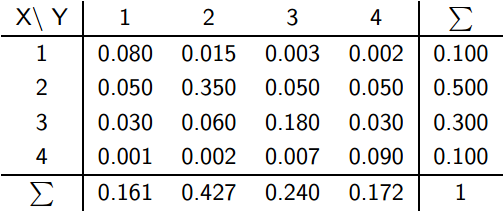
\includegraphics[width=1\linewidth]{images/tableJointDist.png}
				& $P(X=3, Y=4)=0.030$ or $P(X=3 \cup Y=4)=0.030$\vfill
				\vspace*{0.3cm}
				  $P(X=3) = P(X=3, Y=1)+P(X=3, Y=2)+$ \vfill $P(X=3, Y=3)+P(X=3, Y=4) = $\vfill
				  $0.030+0.060+0.180+0.030=0.300$\vfill
				\vspace*{0.3cm}
				$P(Y=2|X=4)=\frac{P(Y=2,X=4)}{P(X=4)}=\frac{0.002}{0.1}=0.02$					\vfill
				\vspace*{0.3cm} 
				$P(X=Y)= P(X=1, Y=1)+P(X=2, Y=2)+$ \vfill $P(X=3, Y=3)+P(X=4, Y=4) = 0.700$\vfill
				\vspace*{0.3cm}
				If random variables are independent it must hold that \vfill
				{$P(X=x, Y=y)=P(X=x) \cdot P(Y=y)$}\vfill
				From the marginal distribution follows \vfill				
				{$P(X=1) \cdot P(Y=2) = 0.100 \cdot 0.427 = 0.043$}			\vfill
				and this is not equal to\vfill
				{$P(X=1, Y=2)= 0.15$}\vfill
				$X$ and $Y$ are \textbf{not independent}\\ 
				\hline
\end{twoColTable}

\begin{twoColTable}
				\hline
				\twoColHdrRow{Joint Density Function}\\
				\hline
				The \textbf{probability} that the \textbf{joint random variable} ($X$,$Y$) lies in a two-dimensional region A, i.e., $A \subset \mathbb{R}^2$, is given by
& $P((X,Y)\in A) = \iint\limits_A f_{X,Y}(x,y)dx\,dy$ \\
The (bivariate) \textbf{joint density function} needs to satisfy& $ \iint\limits_{\mathbb{R}} f_{X,Y}(x,y)dx\,dy = 1$\\
$X$ and $Y$ are only \textbf{independent} if
& $f_{X,Y}(x,y) = f_X(x) \cdot f_Y(y)$, $x,y \in \mathbb{R}$\\
\hline
\textbf{Marginal Density}
& $f_X(x)= \int\limits_{-\infty}^{\infty} f_{X,Y}(x,y) dy$, $f_Y(y)= \int\limits_{-\infty}^{\infty} f_{X,Y}(x,y) dx$\\
\hline
\textbf{Conditional Probability}
& $f_{Y|X=x}(y)=f_Y(y|X=x)=\frac{f_{X,Y}(x,y)}{f_{X}(x)}$\\
$X$ and $Y$ are only independent if the following apply:
&$f_{Y|X=x}(y) = f_Y(y)$ resp. $f_{X|Y=y}(x) = f_X(x)$\\
\hline
\textbf{Conditional Expected Value} of a continuous random variable $Y$ given $X=x$
& $E[Y|X=x]= \int\limits_{-\infty}^{\infty} y \cdot f_{Y|X=x}(y)dy$
\\
\hline
\twoColHdrRow{Example}\\
\hline
Two machines with exponentially distributed life expectancy $X \sim Exp(\lambda_1)$ and $Y \sim Exp(\lambda_2)$, where $X$ and $Y$ are independent. \vfill
$f_X(x) = \lambda_1 e^{-\lambda_1 x}$ and $f_Y(y) = \lambda_2 e^{-\lambda_2 y}$ \vfill
\vspace*{0.3cm}
\centering 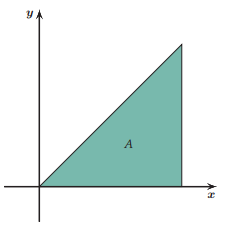
\includegraphics[width=0.5 \linewidth]{images/integrationJointDensityFct.png}
& Due to independence:\vfill
$_{X,Y}(x,y)= \lambda_1 e^{-\lambda_1 x}\lambda_2 e^{-\lambda_2 y}$\vfill
\vspace*{2cm}
$P(Y<X)= \int\limits_0 \limits^{\infty} (\int\limits_0 \limits^{x} \lambda_1 e^{-\lambda_1 x}\lambda_2 e^{-\lambda_2 y} dy)dx$ \vfill
$P(Y<X)= \int\limits_0 \limits^{\infty}  \lambda_1 e^{-\lambda_1 x} (1-e^{-\lambda_2 y})dx = \frac{\lambda_2}{\lambda_1 + \lambda_2}$\\
\hline
\end{twoColTable}
}
\subsubsection{Covariance and Correlation}
{
\setlength{\extrarowheight}{3pt}
		
\begin{twoColTable}
			\hline
			\twoColHdrRow{Covariance and Correlation}\\
			\hline
			\textbf{Covariance}
			& $Cov(X,Y)=E[(X-\mu_X)(Y-\mu_Y)]= E[XY]-E[X]E[Y]$\\
			$X,Y$ independent
			& $E[XY]=E[X]E[Y]$\\
			& $Cov(X,X)=E[(X-\mu_X)(X-\mu_X)] =E[(X-\mu_X)^2] = Var(X) $\\
			Sum of Variances
			& $Var(\sum\limits_{i=1}\limits^{n} X_i)=Cov(\sum\limits_{i=1}\limits^{n} X_i,\sum\limits_{i=1}\limits^{n} X_i)= \sum\limits_{i=1}\limits^{n}Var(X_i)+2\sum\limits_{i<j}\limits^{n} Cov(X_i,X_j)$\\
			2 Random Variables
			& $Var(X+Y)=Cov(X+Y,X+Y)=Var(X)+Var(Y)+2Cov(X,Y)$\\
			If all $X_i$ are independent
			& $Var(X_1 +X_2 +...+X_n)=Var(X_1)+...+Var(X_n)$\\
			\hline
			\textbf{Correlation}
			& $ Cor(X,Y) = \rho_{XY} = \frac{Cov(X,Y}{\rho_X \rho_Y}$ where $-1 \leq Cor(X,Y) \leq 1$\\
			Measure for strength and direction of the \textit{linear dependency} between $X$ and $Y$.
			& $Cor(X,Y)=+1$ if $Y=a+bX$ for $a \in \mathbb{R}$ and $b>0$ \vfill
			$Cor(X,Y)=-1$ if $Y=a+bX$ for $a \in \mathbb{R}$ and $b<0$ 
			\\
			&$|Cor(X,Y)| = 1$ means perfect linear relationship between $X$ and $Y$.\\
			&$Cor(X,Y) = 0$ means $X$ and $Y$ are uncorrelated.\\
			$X$ and $Y$ \textbf{linear independent}
			& $Cor(X,Y) = 0$ (and thus $Cov(X,Y)=0)$\\
			\hline
\end{twoColTable}
		\begin{figure}[H]\centering
			\includegraphics[scale=1]{images/Correlation.png}
			\caption{Correlations}
		\end{figure}
}
\subsubsection{Bivariate Normal Distribution}
{
\begin{twoColTable}
			\hline
			\twoColHdrRow{Bivariate Normal Distribution}\\
			\hline
			Expected values and variances of the marginal distribution
			& $\mu_X, \sigma_X^2$ and $\mu_Y, \sigma_Y^2$\\
			Covariance between $X$ and $Y$
			& $Cov(X,Y)=\rho_{XY}\sigma_X\sigma_Y$\\
			\hline
			Joint Density
			& $f_{X,Y}(x,y)=$\\
			&$\frac{1}{2\pi\sqrt{det(\sum)}}exp\bigg(-\frac{1}{2}(x-\mu_X,y-\mu_Y)\sum^{-1}				\begin{pmatrix}
				x-\mu_X\\
				y-\mu_Y\\
			\end{pmatrix}\bigg)$\\
			\hline
			Covariance Matrix
			& $\sum = \begin{pmatrix}
			Cov(X,X) & Cov(X,Y)\\
			Cov(Y,X) & Cov(Y,Y)\\
			\end{pmatrix}
			= 
			\begin{pmatrix}
			\sigma_X^2 & \rho_{XY}\sigma_X\sigma_Y\\
			\rho_{XY}\sigma_X\sigma_Y & \sigma_Y^2\\
			\end{pmatrix}$\\
			\hline
\end{twoColTable}
}
\subsubsection{Principal Component Analysis (PCA)}
{
PCA is a popular approach for deriving a low-dimensional set of features from a large set of variables. PCA is a technique for reducing the dimension of a $n$ x $p$ data matrix $X$ where $n$ corresponds to the number of observations and $p$ to the number of  variables.
\paragraph{Example: USArrests}
\begin{figure}[H]\centering
\begin{minipage}[c]{0.5\textwidth}
	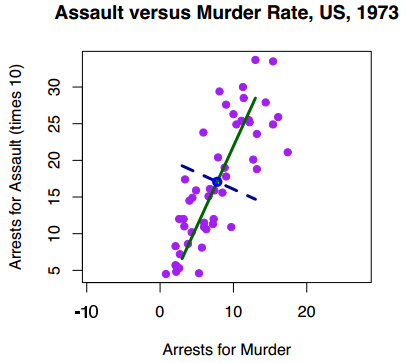
\includegraphics[width=1\linewidth]{images/USArrests_PCA.png}
\end{minipage}\hfill
\begin{minipage}[c]{0.5\textwidth}
	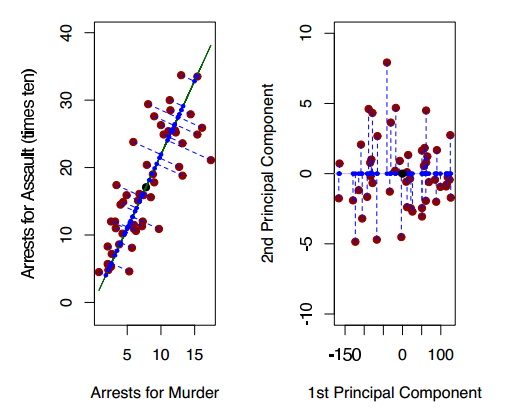
\includegraphics[width=1\linewidth]{images/USArrests_PCA2.png}
\end{minipage}\hfill
\begin{minipage}[t]{.5\textwidth}
	\subcaption{The data vary the most along the first principal component}
\end{minipage}\hfill
\begin{minipage}[t]{.5\textwidth}
	\subcaption{Counter Clockwise Rotation that 1. PC coincides with x-axis}
\end{minipage}
\caption{1st and 2nd Principal Component}
\end{figure}

\begin{figure}[H]\centering
	\begin{minipage}[c]{0.5\textwidth}
		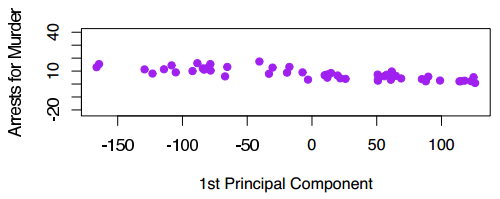
\includegraphics[width=1\linewidth]{images/USArrests_PCA3.png}
	\end{minipage}\hfill
	\begin{minipage}[c]{0.5\textwidth}
		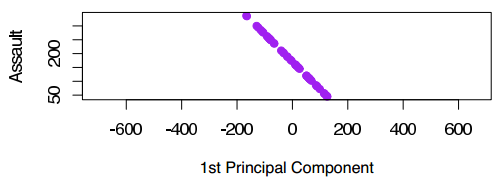
\includegraphics[width=1\linewidth]{images/USArrests_PCA4.png}
	\end{minipage}\hfill
	\begin{minipage}[t]{.5\textwidth}
		\subcaption{$z_{i1}$ versus Murder}
	\end{minipage}\hfill
	\begin{minipage}[t]{.5\textwidth}
		\subcaption{$z_{i1}$ versus Assault}
	\end{minipage}
\end{figure}

\begin{figure}[H]\centering
	\begin{minipage}[c]{0.5\textwidth}
		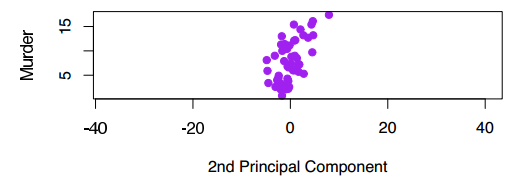
\includegraphics[width=1\linewidth]{images/USArrests_PCA5.png}
	\end{minipage}\hfill
	\begin{minipage}[c]{0.5\textwidth}
		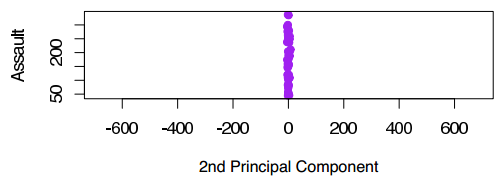
\includegraphics[width=1\linewidth]{images/USArrests_PCA6.png}
	\end{minipage}\hfill
	\begin{minipage}[t]{.5\textwidth}
		\subcaption{$z_{i2}$ versus Murder}
	\end{minipage}\hfill
	\begin{minipage}[t]{.5\textwidth}
		\subcaption{$z_{i2}$ versus Assault}
	\end{minipage}
\caption{The fact that the 2nd principal component scores are much closer to zero indicates that this component captures far less information as the 1st principal component.}
\end{figure}
\RTheory
{	$Z_1=-0.0419126$(Murder - $\overline{\mbox{Murder}})-0.9991213$(Assault-$\overline{\mbox{Assault}})$
	\newline
	\newline
$\phi_{11} = - 0.00419126$ and $\phi_{21} = -0.9991213$ are the \textit{principal component loadings}
\newline
\newline
The idea is that every that out of every linear combination of Murder and Assault sucht that% 
$$\phi_{11}^2+\phi_{21}^2 = 1$$
and \vfill
$$Var(\phi_{11})(\mbox{Murder}-\overline{\mbox{Murder}})+\phi_{21}(\mbox{Assault}-\overline{\mbox{Assault}})$$
is maximized. 
\newline
\newline
{\color{blue}prcomp()} centers the variables to have mean zero. This corresponds to how the first principal component is defined.
\newline
\newline
$z_{i1}=-0.0419126$(Murder - $\overline{\mbox{Murder}})-0.9991213$(Assault-$\overline{\mbox{Assault}})$
\newline
\newline
The values of $z_{i1},...,z_{n1}$ are known as \textit{principal component scores}, seen in the right-hand panel in Figure 6. $z_{i1} > 0$ indicates a state with below-average arrests for murder and below average for assault. A negative score suggests the opposite.
\newline
\newline
	$Z_2=0.9991213$(Murder - $\overline{\mbox{Murder}})-0.0419126$(Assault-$\overline{\mbox{Assault}})$
 }
	{sections/ProbabilityStatistics/JointDistributions/RCode/USArrests_prcomp.R}

	With two-dimensional data, such as in our USArrests example, we can construct at most two principal components. However, if we had other variables, such as Rape, then additional components could be constructed.
	
	\paragraph{PCA and Covariance Matrix}
	{The covariance matrix of two random variables $X$ and $Y$ is defined as 
		$$\sum = 
		\begin{pmatrix}
		Cov(X,X) & Cov(X,Y) \\
		Cov(Y,X) & Cov(Y,Y) \\
		\end{pmatrix}
		=
		\begin{pmatrix}
		\sigma_X^2 & Cov(X,Y) \\
		Cov(Y,X) & \sigma_Y^2 \\
		\end{pmatrix}
	 $$	
	Since $Z_1$ and $Z_2$ are required to be uncorrelated, this implies for their covariance matrix $\sum$ to have vanishing off diagonal elements. Therefore the covariance has to be diagonalized. This can be done with by a rotation matrix $\Phi$ so that
	$$ 
	\begin{pmatrix}
	Z_1\\
	Z_2\\
	\end{pmatrix}
	 = (X-\mu_X,Y-\mu_Y)
	 \begin{pmatrix}
	 \phi_{11}&\phi_{12}\\
	 \phi_{21}&\phi_{22}\\
	 \end{pmatrix}
	 =
	 \begin{pmatrix}
	 \phi_{11}(X-\mu_X)&\phi_{12}(Y-\mu_Y)\\
	 \phi_{21}(X-\mu_X)&\phi_{22}(Y-\mu_Y)\\
	 \end{pmatrix}
	 $$
	 and
	 $$
	 \begin{pmatrix}
	 Cov(Z_1,Z_1)&Cov(Z_1,Z_2)\\
	 Cov(Z_2,Z_1)&Cov(Z_2,Z_2)\\
	 \end{pmatrix}
	 =
	 \begin{pmatrix}
	 	\sigma_{Z_1}^2&0\\
	 	0&\sigma_{Z_2}^2\\
	 \end{pmatrix}
	 $$
	 The rotation matrix $\Phi$ needs to satisfy the condition $\phi_{11}^2+ \phi_{21}^2=1$ and $\phi_{12}^2+\phi_{22}^2=1$
	 It is straightforward to generalize the case of $p=2$ to an arbitrary $p$. 
	}
	\paragraph{Proportion of Variance Explained by Principal Components}
	\RTheory
	{
	There is an information loss of the given data by projecting the observations onto the first few principal components. Therefore we want to know the \textit{proportion of variance explained (PVE)}. The \textit{total variance} is defined as
	$$
	\sum\limits_{j=1}\limits^{p} Var(X_j)=\sum\limits_{j=1}\limits^{p}\frac{1}{n}\sum\limits_{i=1}\limits^{n}x_{ij}^2
	$$	
	and the variance of the $m$th principal component is
	$$
	\frac{1}{n}\sum\limits_{i=1}\limits^{n}z_{im}^2=\frac{1}{n}\sum\limits_{i=1}\limits^{n}\bigg(\sum\limits_{j=1}\limits^{p}\phi_{jm}x_{ij}\bigg)^2
	$$
	Therefore the PVE by the $m$th principal component is given by
	$$
\frac{\sum\limits_{i=1}\limits^{n}\bigg(\sum\limits_{j=1}\limits^{p}\phi_{jm}x_{ij}\bigg)^2}{\sum\limits_{j=1}\limits^{p}\sum\limits_{i=1}\limits^{n}x_{ij}^2}
	$$
	}
	{sections/ProbabilityStatistics/JointDistributions/RCode/USArrests_pve.R}

	


}


\section{Regression Analysis}

\subsection{Simple Linear Regression}

\todo{Chapter 5}

\dots

\subsubsection{Estimating the Coefficients}

\RTheory
	{Estimation of response variable $Y$ based on a predictor variable $X$.%
	$$ Y \simeq \beta_0 + \beta_1X$$}
	{sections/RegressionAnalysis/SimpleLinearRegression/EstimatingCoefficients/theoryCode.R}


\RExample
	{sections/RegressionAnalysis/SimpleLinearRegression/EstimatingCoefficients/exampleCode.R}
	{sections/RegressionAnalysis/SimpleLinearRegression/EstimatingCoefficients/output.R}
	{\todo{interpretation here}}

\subsection{Residual Analysis}

\todo{Chapter 6}
\subsubsection{Diagnostics Instruments}

\input{sections/RegressionAnalysis/ResidualAnalysis/DiagnosticsInstruments/TukeyAnscombe/TukeyAnscombe.tex}
\input{sections/RegressionAnalysis/ResidualAnalysis/DiagnosticsInstruments/ScaleLocation/ScaleLocation.tex}
\input{sections/RegressionAnalysis/ResidualAnalysis/DiagnosticsInstruments/Leverage/Leverage.tex}
\subsection{Multiple Linear Regression}

\todo{Chapter 7}
\subsubsection{Variety of Regression Modelling}
	\paragraph{Omitting Predictor Variables}
		\begin{twoColTable}
			\hline
			\twoColHdrRow{ANOVA Test (Analysis of Variance)}\\
			\hline
			Working principle
				& Based on an $F$-test which provides us with a $p$-value (probability that a value is at least as large as the test statistic)\\
			\hline
			Null hypothesis $H_0$
				& Small model $\mathcal{M}_1$ is sufficient to explain the data.\\
				& I.e. a subset of $q$ coefficients is zero\\
				& $H_0: \quad \beta_{p-q+1} = \beta_{p-q+2} = \dots = \beta_p = 0$\\
			\hline
			Alternative $H_A$
				& A more complex model $\mathcal{M}_2$ is required.\\
			\hline
			RSS of the full model
				& $\mathrm{RSS}$\\
			RSS of the small model
				& $\mathrm{RSS}_0$\\
			$F$-statistic
				& $F = \frac{(\mathrm{RSS_0}-\mathrm{RSS})/q}{\mathrm{RSS}/(n-p-1)}$\\
			\hline
			Conclusion
				& \textbf{Accept the null hypothesis if:}\\
				& $F \approx 1$\\
				& Two-sided $p$-value {\color{blue} Pr($>F$)} $> \alpha$ (significance level)\\
				& \textbf{Reject the null hypothesis if:}\\
				& $F >> 1$\\
				& Two-sided $p$-value {\color{blue} Pr($>F$)} $\leq \alpha$ (significance level)\\
			\hline
		\end{twoColTable}
		
	\paragraph{Example: Omitting predictor variables using {\color{blue}anova()} and {\color{blue}drop1()}}
		\RExample
		{
			sections/RegressionAnalysis/MultipleLinearRegression/VarietyOfRegressionModelling/AnovaDrop1/code.R
		}
		{
			sections/RegressionAnalysis/MultipleLinearRegression/VarietyOfRegressionModelling/AnovaDrop1/Output.R
		}
		{
			\begin{tabular}{>{\bfseries}p{0.13\linewidth}p{0.86\linewidth}}
			First test
				& $F = 0.0312$, $p = 0.8599 >> \alpha$ \textrightarrow\ no evidence to reject the null hypothesis.\\
				& The probability of a measured value of the $F$-statistic to be at least as large as 0.0312, assuming the null hypothesis is true, is very large!\\
			Second test
				& $F = 1076.4$, $p = < 2.2e-16 << \alpha$ \textrightarrow\ reject the null hypothesis.\\
				& The probability of a measured value of the $F$-statistic to be at least as large as 1076.4, assuming the null hypothesis is true, is very small!\\
			Third test
				& For each predictor variable the $F$- and $p$-values are calculated. For TV and radio, the $p$-values are very small, therefore the null hypothesis must be rejected, for newspaper sales, the $p$-value is $>\alpha=5\%$, therefore the null hypothesis must be accepted.\\
				& \note{The {\color{blue}drop1()} function calculates how the quality of a model changes if \underline{only one} predictor is omitted.}
			\end{tabular}
		}
\subsubsection{Collinearity}
	\begin{itemize}
	    \item Collinearity refers to the situation in which two or more predictor variables are closely related to one another. 
	    \item Collinearity causes the standard error of the fitted coefficients to grow.
	    \item Since for the t-statistic, the coefficients are divided by their standard errors, we may fail to reject the null hypothesis.
	\end{itemize}
	
	\paragraph{Variance Inflation Factor (VIF)}
		
		\RTheory
		{
			The ratio of the variance of a coefficient when fitting the full model, divided by the variance of the coefficient when fitted on its own.
			
			$$ \mathrm{VIF}(\beta_j) = \frac{1}{1-R^2_{X_j|X_{-j}}}$$
			
			The minimum value of the VIF is 1, which indicates no collinearity.
			
			\textbf{Rule of thumb:}
			
			A $\mathrm{VIF}>5$ indicates a problematic amount of collinearity
		}
		{
			sections/RegressionAnalysis/MultipleLinearRegression/Collinearity/VIFExample.R
		}
\subsubsection{Qualitative Predictors}
	Qualitative predictors are variables that are used for encoding information other than numeric data. They have discrete levels which indicate information like a country of origin, gender or a profession. They are usually implemented with enumerated data types.
	
	When creating linear models using qualitative predictors, each level (e.g. ``Electrical Engineer'' for the predictor ``Profession'') is assigned their own coefficient.
\subsection{Linear Model Selection}

\todo{Chapter 8}


\clearpage
\input{idiotenseite/IdiotenseiteInclude.tex}

\end{document}
